\documentclass[notheorems,11pt,compress]{beamer}


%------ Beamer theme ------
%\usetheme{Frankfurt}
%\usetheme{Montpellier}
%\usetheme{Warsaw}
%\usetheme{CambridgeUS}
%\usetheme{Boadilla}

%------- Color theme ------
\usecolortheme{rose}
%\usecolortheme{orchid}
%\usecolortheme{lily}
%\usecolortheme{whale}
%\usecolortheme{dolphin}
%\usecolortheme{seahorse}

%\usetheme{boxes}
%\setbeamercovered{transparent}
%\usefonttheme[onlymath]{serif}
\usefonttheme{serif}
\usefonttheme{professionalfonts}

%\setbeamertemplate{headline}{}
%\setbeamertemplate{footline}{}
\setbeamertemplate{blocks}[rounded][shadow=true]
\setbeamertemplate{navigation symbols}{}
\setbeamertemplate{itemize items}[circle]  % ball, circle
\setbeamertemplate{enumerate items}[default]
%\setbeamertemplate{section in toc}[square]
\setbeamertemplate{section in toc}
{\leavevmode\leftskip=2.5em%
	\llap{%
		\usebeamerfont*{section number projected}%
		\usebeamercolor{section number projected}%
		\begin{pgfpicture}{-1ex}{0ex}{1ex}{2ex}
			\color{darkorange}
			\pgfpathcircle{\pgfpoint{0pt}{.75ex}}{1.3ex}
			\pgfusepath{fill}
			\pgftext[base]{\color{fg}\inserttocsectionnumber}
		\end{pgfpicture}\kern1.25ex%
	}%
	\inserttocsection\par
}


\setbeamersize{text margin left=0.5cm, text margin right=0.5cm}

\definecolor{darkblue}{rgb}{0.02,0.24,0.44}
\definecolor{darkorange}{rgb}{0.80,0.4,0.1}
\definecolor{lightgray}{rgb}{0.78,0.78,0.78}
\definecolor{darkgray}{rgb}{0.30,0.30,0.30}
\definecolor{darkgreen}{rgb}{0.02,0.18,0.20}
\definecolor{footer}{rgb}{0.5,0.2,0.5}

\setbeamercolor{frametitle}{fg=darkblue,bg=black!5}
\setbeamercolor{section in head/foot}{bg=black,fg=darkorange}
\setbeamercolor{lower separation line head}{bg=darkblue}
\setbeamertemplate{section in head/foot shaded}{\color{lightgray}
	\usebeamertemplate{section in head/foot}}

\setbeamercolor{title in head/foot}{bg=darkgreen,fg=black!5}
\setbeamercolor{section in toc}{fg=darkorange}

\setbeamercolor{structure}{fg=darkblue}
\setbeamercolor{alerted text}{fg=darkorange}

%\setbeamertemplate{section in toc}[sections numbered]
%\setbeamertemplate{subsection in toc}[subsections numbered]
%\setbeamertemplate{section in toc}[ball unnumbered]
%\setbeamertemplate{subsection in toc}[ball unnumbered]

% change the style of headline
\setbeamertemplate{headline}{
	\begin{beamercolorbox}[ht=4.5ex]{section in head/foot} %,dp=0.0ex
		\vskip2pt\insertsectionnavigationhorizontal{\textwidth}{}{}\vskip2pt
		%\vskip2pt\insertnavigation{\paperwidth}\vskip2pt
	\end{beamercolorbox}
	\begin{beamercolorbox}[colsep=1.5pt]{lower separation line head} %
	\end{beamercolorbox}
}



\setbeamertemplate{frametitle}{%
	\nointerlineskip%
	\begin{beamercolorbox}[wd=\paperwidth,ht=2.75ex,dp=1ex]{frametitle}
		\hspace*{1.5ex}\insertframetitle%
	\end{beamercolorbox}%
	%\vspace*{-1ex}
}


\setbeamertemplate{footline}
{%
	\leavevmode%
	\begin{beamercolorbox}[wd=0.25\paperwidth,ht=2.5ex,dp=1.125ex,leftskip=.3cm,rightskip=.3cm plus1fil]{title in head/foot}%
		\usebeamerfont{title in head/foot} ~~\insertshortauthor~(\insertshortinstitute) \hfill
	\end{beamercolorbox}%
	\begin{beamercolorbox}[wd=0.5\paperwidth,ht=2.5ex,dp=1.125ex,leftskip=.3cm,rightskip=.3cm plus1fil]{title in head/foot}%
		\usebeamerfont{title in head/foot}\centering \insertshorttitle
	\end{beamercolorbox}%
	\begin{beamercolorbox}[wd=0.25\paperwidth,ht=2.5ex,dp=1.125ex,leftskip=.3cm,rightskip=.3cm plus1fil]{title in head/foot}%
		\usebeamerfont{title in head/foot} \hfill
		\insertframenumber\,/\,\inserttotalframenumber\kern2pt
	\end{beamercolorbox}%
	\vskip0pt%
}


%--------- 宏包  ----------
\usepackage[UTF8,noindent]{ctex}
%\usepackage[english]{babel}
\usepackage{amsmath,amssymb,version}
\usepackage{ulem}
\usepackage{graphicx,fancybox,mathrsfs,multirow}
\usepackage{booktabs}
\usepackage{epsfig,epstopdf}
\usepackage{url,hyperref}
% \bibliographystyle{apacite}
\usepackage{float}
\usepackage{tabularx,array,makecell}
\usepackage{color,xcolor}
\usepackage{cases}
\usepackage{tcolorbox}
\usepackage{mathtools}
\usepackage{tikz}
\usepackage[
	natbib=true,
	% style=authoryear,
	backend=bibtex,
	useprefix=true]{biblatex}
\addbibresource{refs.bib}
%---------- 定义行距 ----------
%\renewcommand{\baselinestretch}{1.15}

%---------- 定义表格新命令 ----------
\newcolumntype{P}[1]{>{\centering \arraybackslash}p{#1}}
\newcolumntype{L}{X}
\newcolumntype{C}{>{\centering \arraybackslash}X}
\newcolumntype{R}{>{\raggedleft \arraybackslash}X}

%---------- 设置字体  ----------
\setbeamerfont{normal text}{family=\rmfamily}
\setbeamerfont{frametitle}{family=\rmfamily,series=\bfseries}
\setbeamerfont{title}{family=\sffamily}
\setbeamerfont{subtitle}{family=\sffamily}
\setbeamerfont{institute}{family=\rmfamily}
\setbeamerfont{author}{family=\rmfamily}
\setbeamerfont{date}{family=\rmfamily}
\setbeamerfont{headline}{family=\sffamily} %,series=\bfseries
\setbeamerfont{footline}{family=\sffamily} %\kaishu
\setbeamerfont{section in toc}{family=\rmfamily}
\setbeamerfont{subsection in toc}{family=\rmfamily}
\AtBeginDocument{\usebeamerfont{normal text}}

\setbeamercolor{title}{fg=darkblue,bg=black!10}
\setbeamercolor{subtitle}{fg=darkblue!80}
%\setbeamercolor{institute}{fg=white}
%\setbeamercolor{author}{fg=white}
%\setbeamercolor{date}{fg=white}

\setbeamertemplate{caption}[numbered]
\numberwithin{figure}{section}
\numberwithin{table}{section}
\numberwithin{equation}{section}


%---------- 定理设置  --------------
\theoremstyle{plain}
\setbeamertemplate{theorems}[numbered]
\addtobeamertemplate{theorem begin}{\normalfont}{}
%\theoremstyle{definition}
%\newtheorem{theorem}{Theorem}
\newtheorem{theorem}{定理} %\sffamily
\numberwithin{theorem}{section}
%\newtheorem{definition}{Definition}
\newtheorem{definition}{定义}
\numberwithin{definition}{section}
%\newtheorem{lemma}{Lemma}
\newtheorem{lemma}{引理}
\numberwithin{lemma}{section}
%\newtheorem{proposition}{Proposition}
\newtheorem{proposition}{命题}
\numberwithin{proposition}{section}
%\newtheorem{corollary}{Corollary}
\newtheorem{corollary}{引理}
\numberwithin{corollary}{section}
\theoremstyle{example}
%\newtheorem{example}{Example}
\newtheorem{example}{例}
%\numberwithin{example}{section}
\renewenvironment{proof}[1][证明]{\textbf{#1}:~~}{\qed\par}
\newenvironment{solution}{\par\noindent\textbf{解}:~~}{\par}


%---------- 调节公式的间距 ----------
%\AtBeginDocument{
%	\setlength{\abovedisplayskip}{4pt plus 1pt minus 1pt}
%	\setlength{\belowdisplayskip}{4pt plus 1pt minus 1pt}
%	\setlength{\abovedisplayshortskip}{2pt}
%	\setlength{\belowdisplayshortskip}{2pt}
%	\setlength{\arraycolsep}{2pt}
%}


\makeatletter
\newcommand\HUGE{\@setfontsize\Huge{28}{32}}
\makeatother


% \AtBeginSection[]{
% \begin{frame}
%  \frametitle{Content}
%  \tableofcontents[currentsection,currentsubsection,subsectionstyle=show/show/shaded]
%  \addtocounter{framenumber}{-1}
% \end{frame}
% }

\AtBeginSection[]
{
	\begin{frame}<beamer>
		\frametitle{\textbf{Content}}
		\tableofcontents[currentsection,currentsubsection]
	\end{frame}
}

%---------- 自定义命令 ----------
\newcommand{\red}[1]{\textcolor{red}{#1}}
\newcommand{\blue}[1]{\textcolor{blue}{#1}}
\newcommand{\upcite}[1]{\textsuperscript{\cite{#1}}}

%--------------------------------------------------------------------------------
%	TITLE PAGE
%--------------------------------------------------------------------------------


\title[复杂系统建模论文报告]{复杂系统建模论文报告
	\\[8pt] Defectors in bad circumstances possessing
	\\[5pt] higher reputation can promote cooperation}

\author[X]{X}
\institute[DLUT]{\vskip -10pt
	\small {大连理工大学数学系}
	\vskip 10pt
}

\date[2022.10.14]{2022\,年\,10\,月\,14\,日}
% \date[\today]{\today}


\graphicspath{{./figs/}}


\begin{document}

% only change the spacing of body text
\setlength{\baselineskip}{15pt}


{%\setbeamertemplate{headline}{}
	\begin{frame}
		\titlepage % Print the title page as the first slide
	\end{frame}}


\begin{frame}
	\frametitle{\textbf{Content}}
	\tableofcontents
\end{frame}


%--------------------------------------------------------------------------------
%	PRESENTATION SLIDES
%--------------------------------------------------------------------------------
\begin{frame}
	\begin{figure}[H]
		\centering
		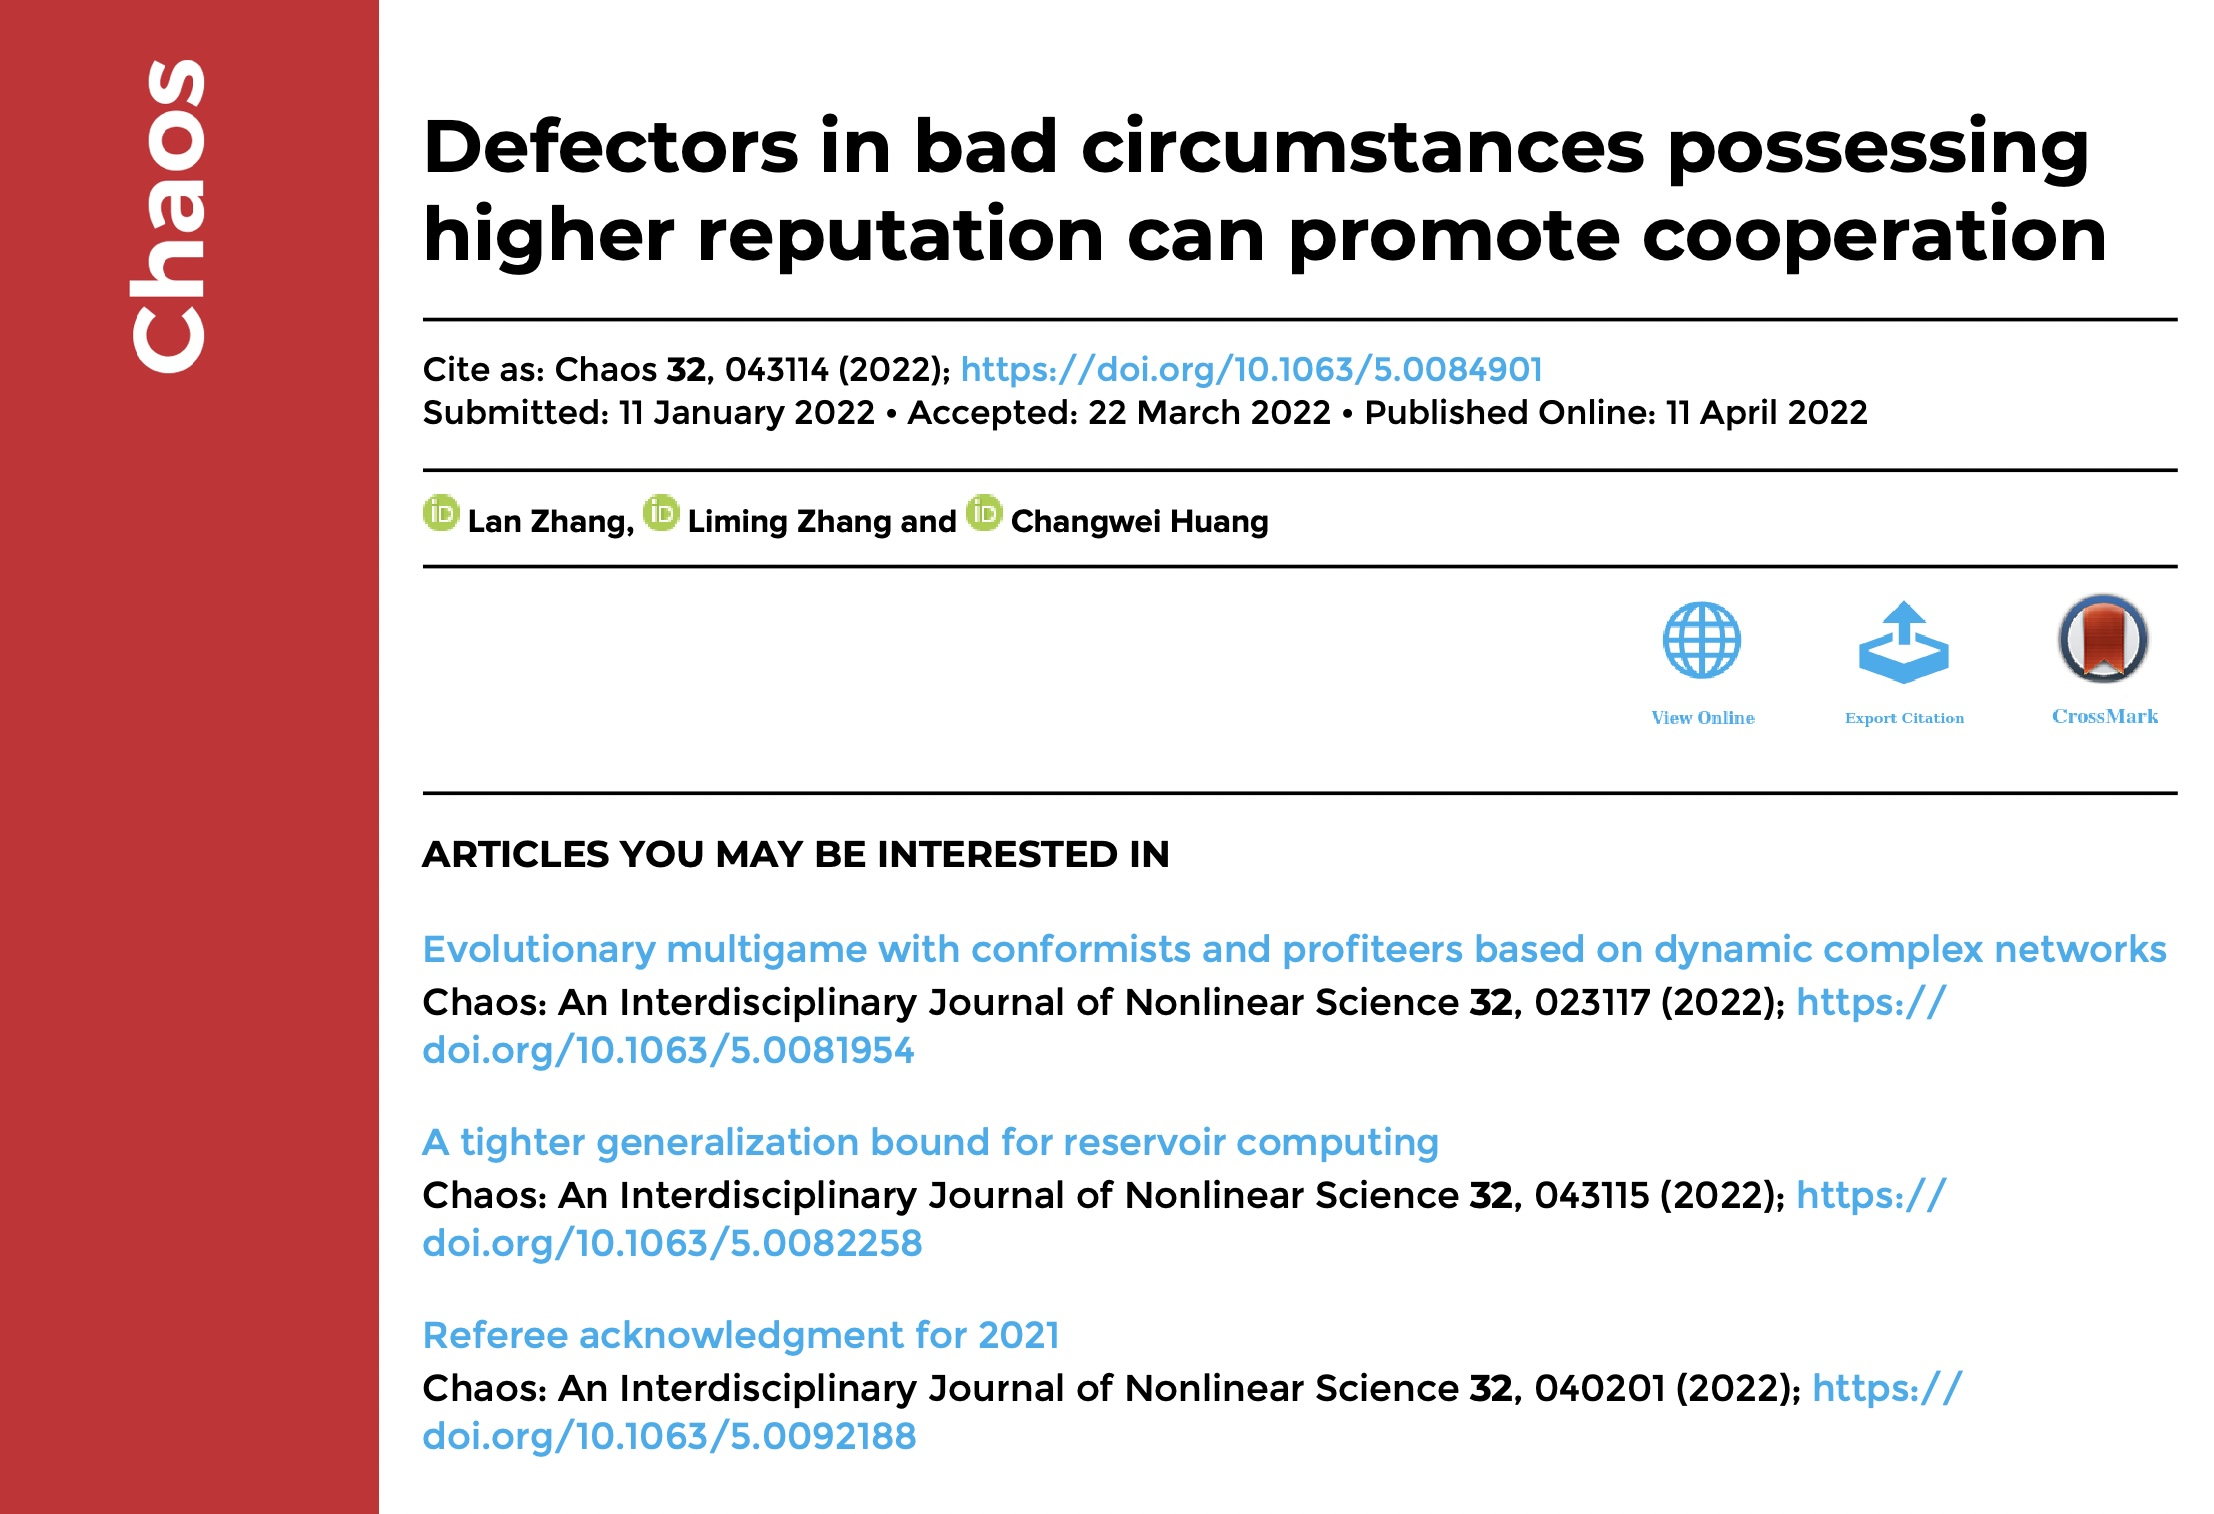
\includegraphics[width=1\textwidth]{paper}
	\end{figure}
\end{frame}
%------------------------------------------------
\section{Background,Method and Significance}
%------------------------------------------------

\begin{frame}{Research background}


	In nature and human society, social relationships and behavior patterns are usually unpredictable.
	The concept of ``\underline{reputation}'' can provide some information to mitigate(means weaken) such uncertainty.

	\vspace{1ex}

	In previous studies, researchers have considered that only \textbf{cooperators} are able to maintain a high reputation.

	In reality, however, some individuals will be forced to defect to protect themselves against exploitation.
	Therefore, \textbf{defectors in bad circumstances} could also obtain higher reputations, and cooperators can maintain higher reputations in comfortable circumstances.

\end{frame}

%-----------------------------------------------

\begin{frame}{Research Method}

	In this work, the reputations of individuals are calculated using the \textbf{fraction of their neighbors who have the same strategy}. Therefore, some defectors in a population may obtain higher reputations than some cooperators.

	\begin{exampleblock}{Research process and method}
		\begin{itemize}
			\item The reputation rule using \textbf{heterogeneous investments in public goods games}.
			\item Dynamical evolution is observed in \textit{Monte Carlo simulations}.
			\item The effects of the noise intensity of the irrational population and the original proportion of cooperation in the population.
			\item Use numerical simulation to indicate conclusions.
		\end{itemize}
	\end{exampleblock}

\end{frame}

%------------------------------------------------

\begin{frame}{Research significance}


	\begin{alertblock}{Main results and research significance}
		\begin{enumerate}
			\item The reputation rule and heterogeneous investments can better stimulate cooperation.
			      \vspace*{1ex}
			\item Stronger investment heterogeneity can further increase the level of cooperation.
			      \vspace*{1ex}
			\item The conclusion is the same when we consider network structure and total investment.
		\end{enumerate}
	\end{alertblock}


\end{frame}

%------------------------------------------------
\section{Preliminary}

\begin{frame}{Preliminary}

	\begin{alertblock}{}
		\begin{itemize}
			\item Theory of game.
			\item Spatial PGG(Public Goods Game) model.
			\item Barabási–Albert (BA) scale-free network.
			\item Monte Carlo simulations.
			\item Fermi rule.
			\item Numerical simulation by \textbf{Fortran}.
		\end{itemize}
	\end{alertblock}
\end{frame}

%------------------------------------------------

\begin{frame}{PGG model}
	\begin{block}{PGG model}
		The public goods game(PGG)\upcite{wiki:pgg} is a standard of experimental economics.
		In the basic game, subjects secretly choose how many of their private tokens to put into a public pot.
		The tokens in this pot are multiplied by a factor (greater than one and less than the number of players, N) and this ``public good'' payoff is evenly divided among players.
		Each subject also keeps the tokens they do not contribute.
	\end{block}
	\vspace*{2em}

\end{frame}

%------------------------------------------------

\begin{frame}{Barabási–Albert (BA) model}
	\begin{block}{BA model}
		The Barabási–Albert (BA)\upcite{wiki:ba} model is an algorithm for generating random scale-free networks using a preferential attachment mechanism.

		Several natural and human-made systems, including the Internet, the World Wide Web, citation networks, and some social networks are thought to be approximately scale-free and certainly contain few nodes (called hubs) with unusually high degree as compared to the other nodes of the network.
	\end{block}
	\vspace*{2em}

\end{frame}
%------------------------------------------------


%------------------------------------------------
\section{Contents} % XX 方法求解  XX 方程
%------------------------------------------------


\begin{frame}{Paper Structure}
	\begin{enumerate}
		\item the reputation rule and the \textit{spatial PGG model}
		\item the results of numerical simulations
		\item summarizes the paper and puts forward directions for future research
	\end{enumerate}
\end{frame}
%------------------------------------------------


\begin{frame}{Research hypothesis}  % Multiple Columns

	% \begin{columns}[t] % The "c" option specifies centered vertical alignment while the "t" option is used for top vertical alignment

	% \column{.45\textwidth} % Left column and width
	% \textbf{Heading}
	\begin{enumerate}
		\item An individual’s reputation may reflect the willingness of their neighbors to cooperate with them.
		      \vspace*{1ex}
		\item Most previous studies of reputation have assumed that social interactions are public, which means that everyone knows about the details of these interactions.
		      \vspace*{1ex}
		\item $\bigstar$ Some individuals in bad circumstances will be forced to defect to protect themselves against exploitation.
		      \vspace*{1ex}
		\item A cooperator (defector) with more cooperative (defective) neighbors can obtain a higher reputation.
	\end{enumerate}

	% \column{.5\textwidth} % Right column and width
	% The quick brown fox jumps over the lazy dog. The quick brown fox jumps over the lazy dog. The quick brown fox jumps over the lazy dog. The quick brown fox jumps over the lazy dog.
	% \end{columns}
\end{frame}
%------------------------------------------------

\subsection{The reputation rule}
\begin{frame}{The reputation rule}
	The reputation $R_i(t)\in[0,1]$ of individual $i$ at step $t$:
	\begin{equation}
		R_i(t)= \begin{cases}\dfrac{N_i(t-1)}{k_i(t-1)} & \text { if } s_i(t-1)=1, \\ 1-\dfrac{N_i(t-1)}{k_i(t-1)} & \text { if } s_i(t-1)=0.\end{cases}
	\end{equation}

	where
	\begin{itemize}
		\item $N_i(t-1)$: the number of cooperators among the neighbors of individual $i$ at step $t-1$;
		\item $k_i$: the degree of individual $i$;
		\item $s_i$: the strategy of individual $i$($s_i=1$ if individual $i$ is a cooperator,otherwise $s_i=0$).
	\end{itemize}

\end{frame}

%------------------------------------------------

\begin{frame}{Spatial PGGs in structured populations}

	Consider a $L\times L$ square lattice with periodic boundary conditions.
	Each individual is located on a single node surrounded by four nearest neighbors.

	In a square lattice, there are five different reputation levels.

	The possible reputation values for each individual are $\left[0,1/4,1/2,3/4,1\right]$.

	Also consider a lattice with eight nearest neighbors and the Barabási–Albert (BA) scale-free network.

\end{frame}

\subsection{Monte Carlo simulations}

\begin{frame}{Monte Carlo simulations}
	\begin{exampleblock}{Three elementary procedures}
		\begin{enumerate}
			\item investment allocation;
			\item payoff accumulation;
			\item strategy updating.
		\end{enumerate}
	\end{exampleblock}
\end{frame}


%------------------------------------------------

\begin{frame}{investment allocation}

	The total investments $c$ of each cooperator are equal and $c = 1$.

	In contrast to the traditional PGG, define \textbf{heterogeneous investments induced by reputation}.

	At step $t$, $I_{i\to j}(t)$ is the investment in the group organized by individual $j$ from cooperator $i$.
\end{frame}



\begin{frame}{investment allocation}

	\begin{equation}\label{eq2}
		I_{i \rightarrow j}(t)=c \cdot \frac{e^{\alpha \cdot R_j(t-1)}}{\sum_{k \in \Omega_i} e^{\alpha \cdot R_k(t-1)}}
	\end{equation}

	where
	\begin{itemize}
		\item $\Omega_i$: the collection of individual i and its neighbors;
		\item $\alpha(\alpha\geq0)$: a tunable parameter controlling the strength of investment heterogeneity.
	\end{itemize}

	When $\alpha  = 0$, the model collapses to the traditional PGG, in which cooperators invest in all common pools with no differences.
\end{frame}


\begin{frame}{investment allocation}

	The detailed calculation of the investment using Eq~\ref{eq2} starts at the second step.

	All investments $I_{i\to j}$ take a value of $0.2$ at the first step.
	In real life, individuals tend to invest more in other individuals with higher reputations, this corresponds to the case of $\alpha >0$.

	A defector with only one cooperative neighbor is also considered to have a better reputation; the cooperative neighbor will be willing to provide certain help to the benefit of this defector.
\end{frame}


\begin{frame}{investment allocation}

	In Eq~\ref{eq2}, $\alpha $ is a key parameter to distinguish from the tradition PGG.
	To better demonstrate the impact of $\alpha $ on the investment, we measure the investment heterogeneity of an individual by calculating the variance of the investment $\sigma_{I_{i\to j}}$.

	\begin{equation}\label{eq3}
		\sigma_{I_{i \rightarrow j}}=\frac{1}{G} \sum_{k \in \Omega_i}\left(I_{i \rightarrow k}-\frac{c}{G}\right)^2,
	\end{equation}

	where

	\begin{itemize}
		\item $G$: the number of individuals in one group;
		\item $\alpha(\alpha\geq0)$: a tunable parameter controlling the strength of investment heterogeneity.
	\end{itemize}
\end{frame}


\begin{frame}{investment allocation}

	\begin{figure}[H]
		\centering
		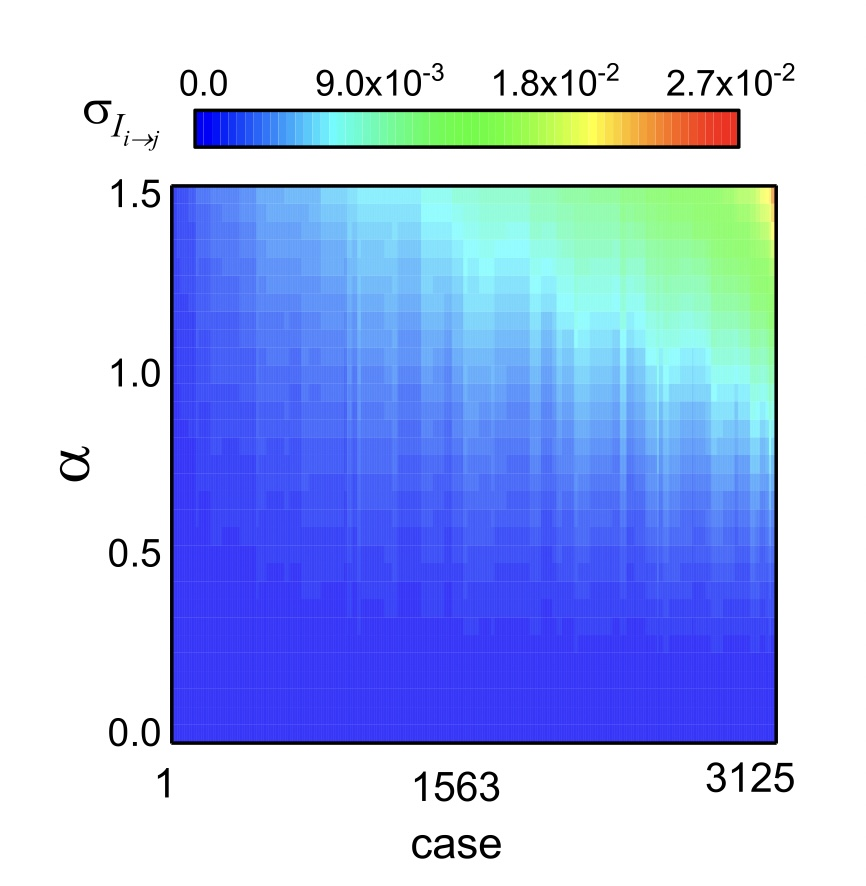
\includegraphics[width=0.5\linewidth]{1a}
		\quad
		\parbox[b]{.45\textwidth}{
			In the left several columns, all $\sigma_{I_{i \rightarrow j}}=0$ whatever $\alpha$ is because of the same reputation of all group members and $I_{i\to j} = 0.2$. Except for the several columns, $\sigma_{I_{i \rightarrow j}}$ grows with increasing $\alpha$ in the other cases.\uline{The investment heterogeneity of an individual becomes stronger as $\alpha$ increases as long as the reputations are not identical. }}
		\parbox{.75\textwidth}{\vspace*{1ex}Fig\ 1a: Color map of the investment heterogeneity $\sigma_{I_{i \rightarrow j}}$ in the $\alpha$ and case space}
		\label{fig1a}
	\end{figure}
\end{frame}


\begin{frame}{investment allocation}
	Calculate the mean of the investment variances for all individuals in a square lattice with the random initial condition:
	\begin{equation}
		\bar{\sigma}_{I_{i \rightarrow j}}=\frac{1}{N} \sum_{i=1}^N \sigma_{I_{i \rightarrow j}},
	\end{equation}

	\begin{figure}[H]
		\centering
		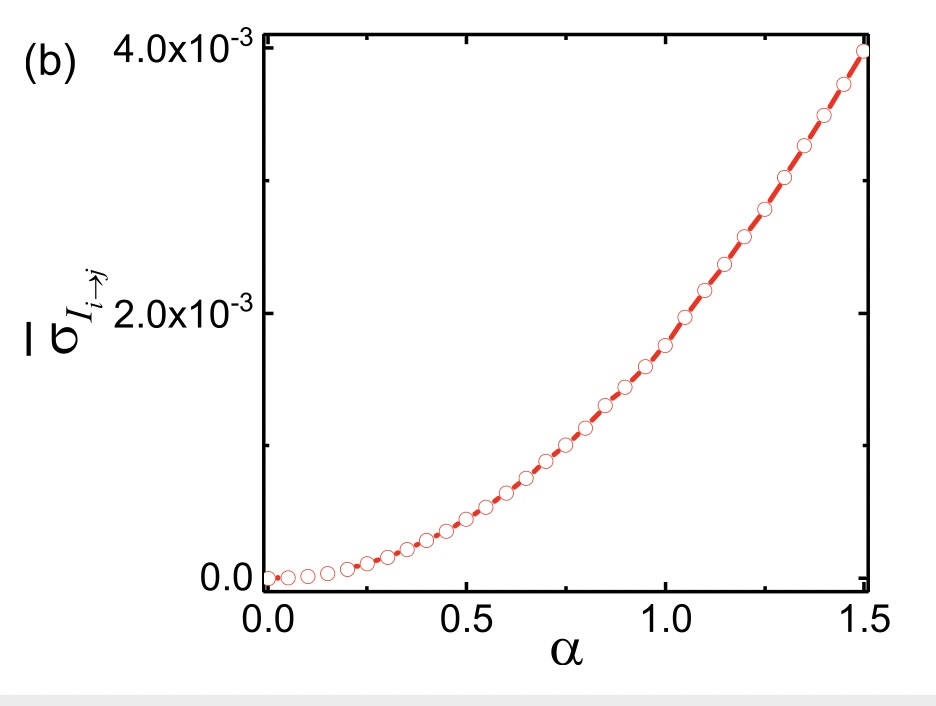
\includegraphics[width=0.52\linewidth]{1b}
		\,
		\parbox[b]{.45\textwidth}{Fig\ 1b: \ The relationship between the investment heterogeneity $\sigma_{I_{i \rightarrow j}}$ calculated at step $t = 2$ and $\alpha$. Simulations are carried out for the square lattice.\vspace*{3em}}
		\label{fig1b}
	\end{figure}
\end{frame}

%------------------------------------------------

\begin{frame}{payoff accumulation}

	The payoff of individual $i$ at step $t$ can be calculated from
	\begin{equation}
		U_i(t)=\frac{r}{G} \sum_{j \in \Omega_i} \sum_{k \in \Omega_j} I_{k \rightarrow j}(t)-s_i(t) \cdot c.
	\end{equation}

\end{frame}


%------------------------------------------------

\begin{frame}{strategy updating}

	Use the \textbf{Fermi rule} as the strategy-update rule. In each step, each individual $i$ randomly selects a neighbor $j$. Then, $i$ learns the strategy of $j$ with a probability $P$ calculated by the Fermi function:

	\begin{equation}
		P\left(s_j \rightarrow s_i\right)(t)=\frac{1}{1+\exp \left[\left(U_i(t)-U_j(t)\right) / \kappa\right]},
	\end{equation}
	\begin{block}{}
		$\kappa$: the noise intensity of the irrational population, $\kappa$ is set as $0.1$ in this work.
		\begin{itemize}
			\item $\kappa\to0$: individual $i$ will adopt the strategy of individual $j$ as long as $j$ has a higher payoff.
			\item $\kappa\to+\infty$: random section.
		\end{itemize}
	\end{block}
\end{frame}




%------------------------------------------------
\section{Numerical Simulation}
%------------------------------------------------

\begin{frame}{Numerical simulation}

	All simulation results are obtained on lattice comprising $N = 100 \times 100$ individuals or a BA scale-free network comprising $N = 3000$ individuals. At the beginning of each simulation, individuals choose one of the strategies of cooperation and defection randomly.

	Monitor key quality $f_C$ measures the cooperation frequency in the population.

	Calculate $f_C$ within the last $3000$ steps of a total of $2 \times 10^4$ steps.


\end{frame}


% \begin{table}
% \caption{这是一个三线表.}
% \begin{tabular}{lll}
% \toprule
% \textbf{Treatments} & \textbf{Response 1} & \textbf{Response 2}\\
% \midrule
% Treatment 1 & 0.0003262 & 0.562 \\
% Treatment 2 & 0.0015681 & 0.910 \\
% \bottomrule
% \end{tabular}
% \end{table}



%------------------------------------------------
\subsection{Cooperative behavior in a square lattice}

\begin{frame}{Cooperative behavior in a square lattice}

	\begin{figure}[H]
		\centering
		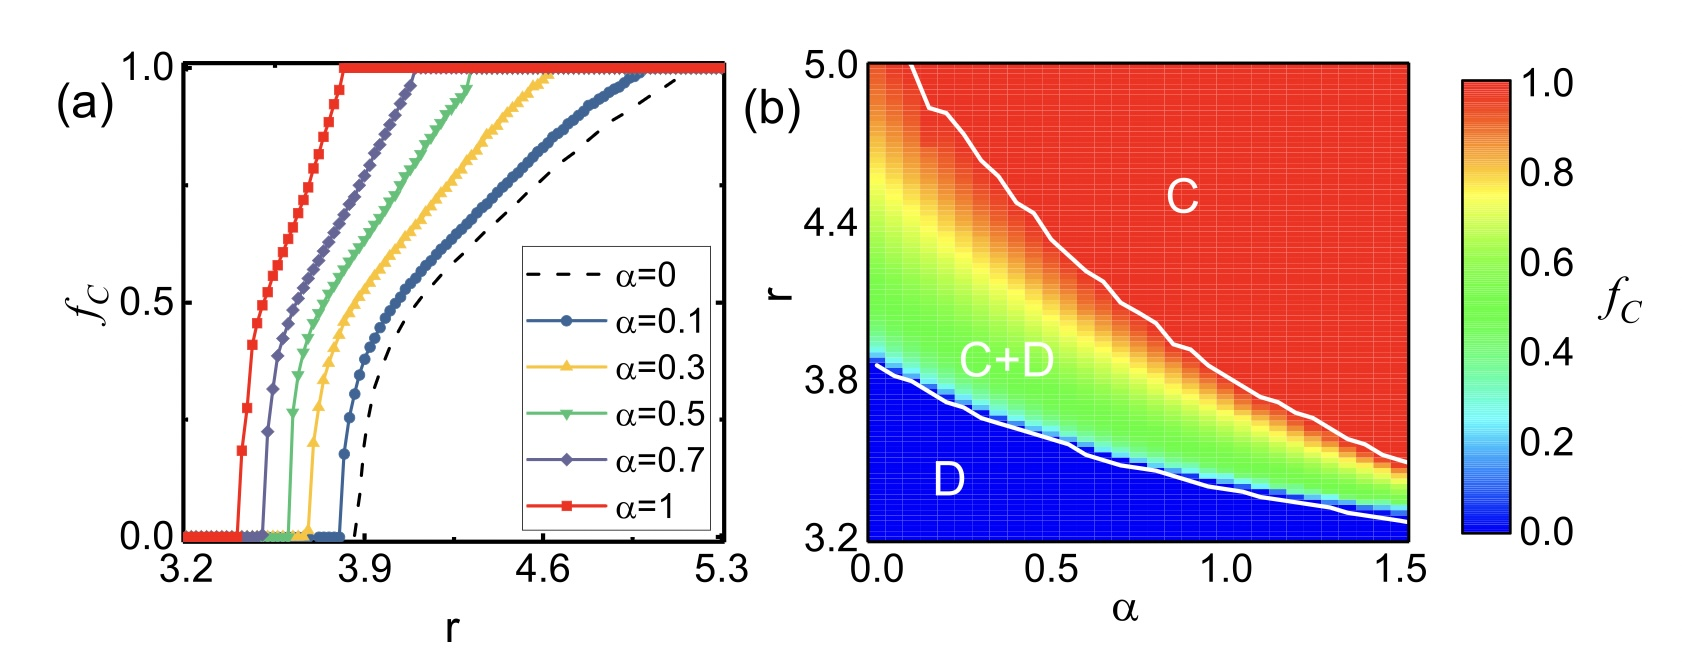
\includegraphics[width=1\linewidth]{2}
		\parbox{.8\textwidth}{Fig\ 2:(a) Relationship between the cooperation frequency $f_C$ and the synergy factor $r$ at several heterogeneity strengths $\alpha$.
			(b) Color map of the cooperation frequency $f_C$ in the $r–\alpha$ parameter space.
			The white curves denote the critical values $r_{c1}$ (lower) and $r_{c2}$ (upper).}
		\label{fig2}
	\end{figure}
\end{frame}


\subsection{Dynamical evolution of cooperation
}
\begin{frame}{Dynamical evolution of cooperation
	}
	\begin{figure}[H]
		\centering
		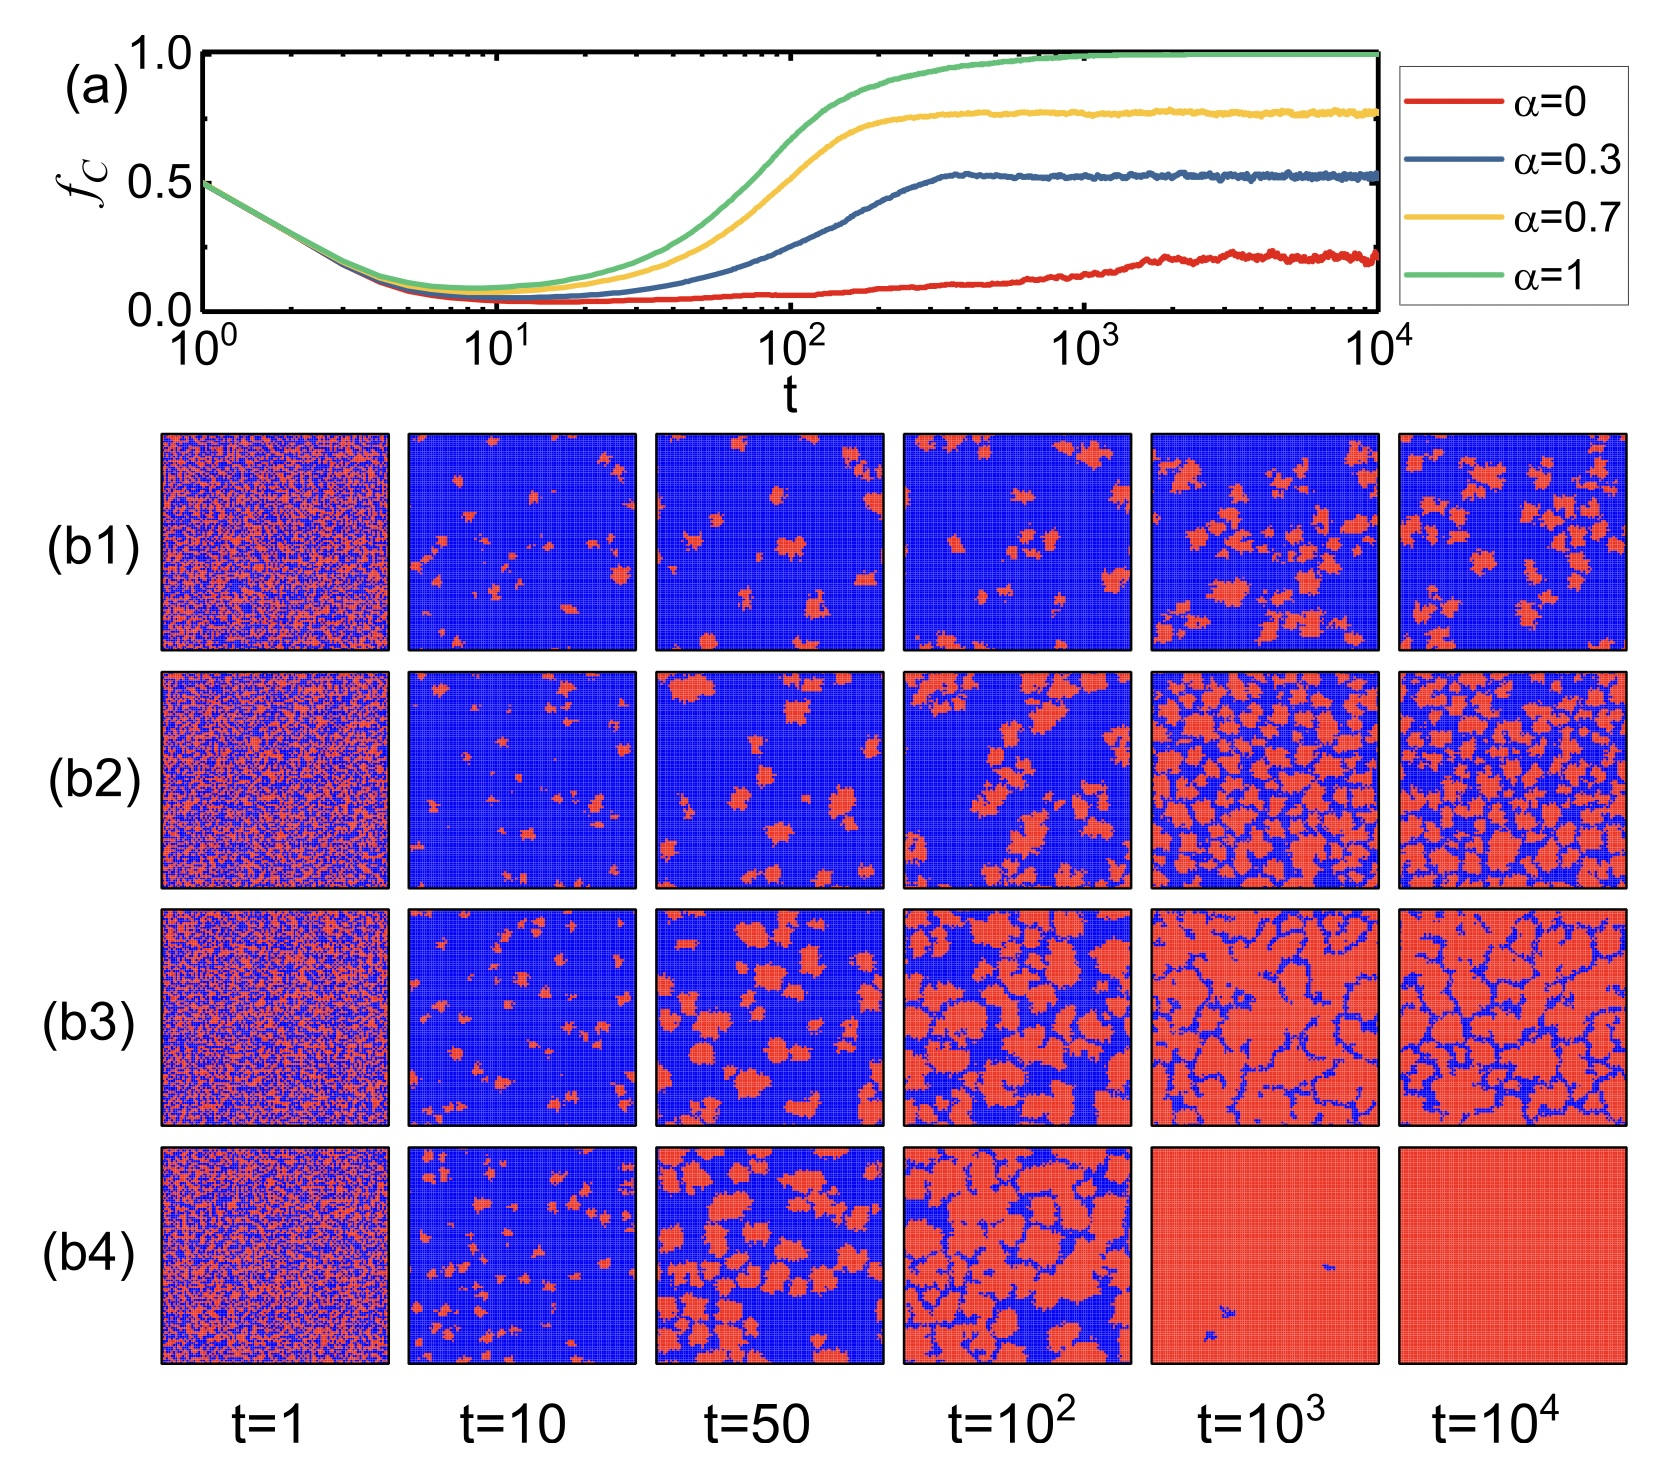
\includegraphics[width=.65\linewidth]{3}
		\label{fig3}
		\,
		\parbox{.3\textwidth}{\scriptsize Fig\ 3 :(a) Time courses of the cooperation frequency $f_C$ with several $\alpha$ values. (b1)–(b4) Snapshots of the distributions of cooperators (red) and defectors (blue) at several typical time nodes: (b1) $\alpha = 0$, (b2) $\alpha = 0.3$, (b3) $\alpha = 0.7$, and (b4) $\alpha = 1.0$. In all cases, $r = 3.9$.
			\vspace*{10em}
		}
	\end{figure}
\end{frame}


\begin{frame}{Dynamical evolution of cooperation
	}


	\begin{figure}[H]
		\centering
		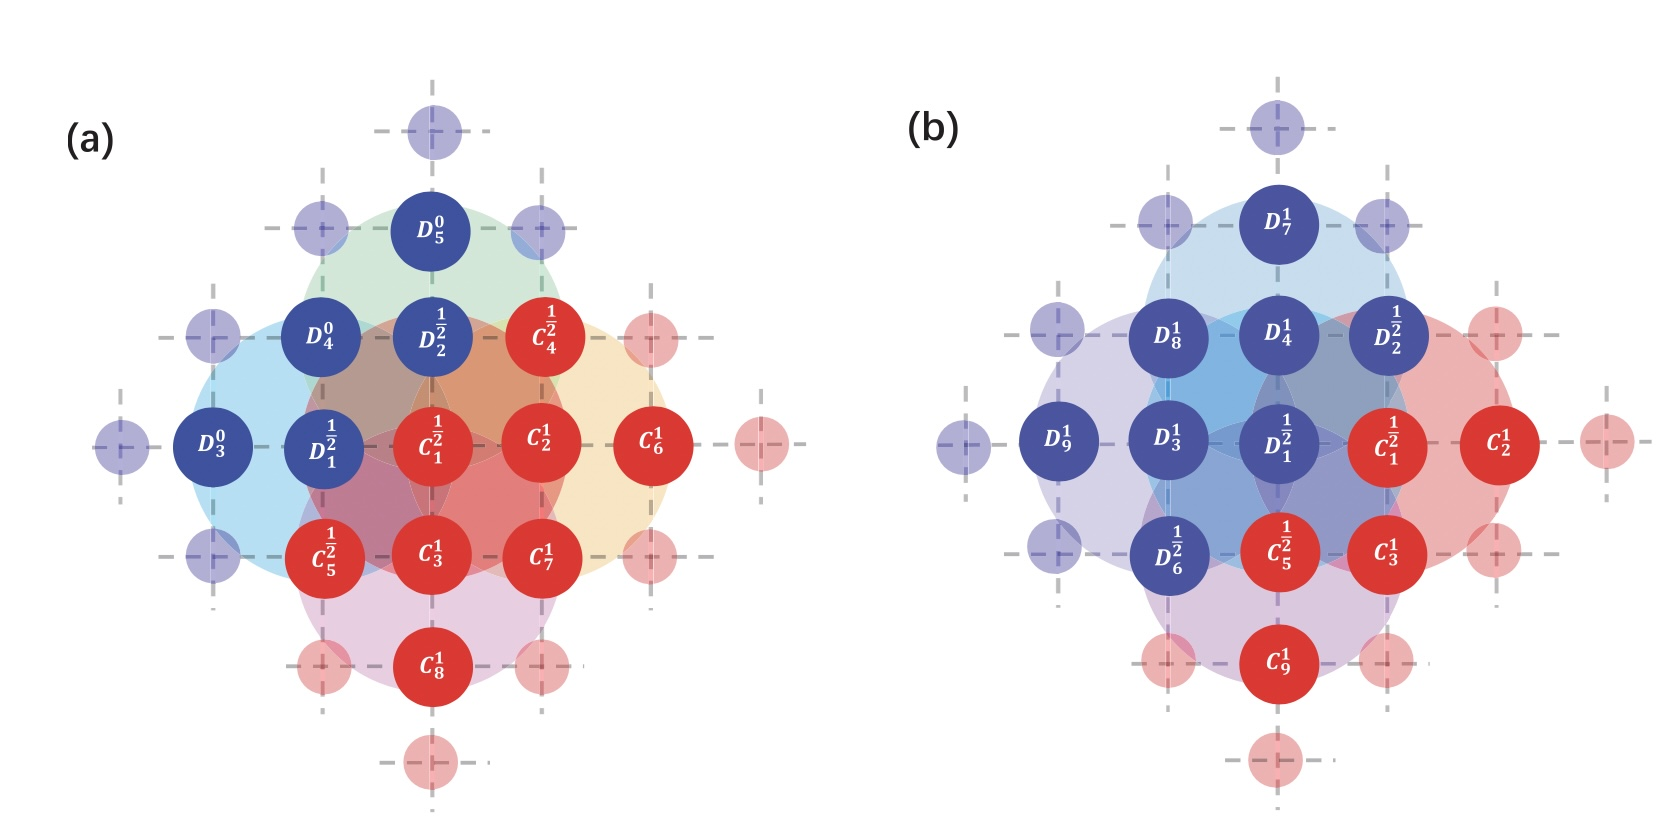
\includegraphics[width=1\linewidth]{4}
		\label{fig4}
		\parbox{.8\textwidth}{\scriptsize Fig\ 4: PGGs staged on the edges of C-clusters. (a) PGG focused on a cooperator. (b) PGG focused on a defector. Red and blue points represent cooperators and defectors, respectively. The subscripts denote the serial numbers of individuals, and their corresponding reputations are shown by superscripts.
		}
	\end{figure}
\end{frame}


\begin{frame}{Dynamical evolution of cooperation
	}
	\begin{figure}[H]
		\centering
		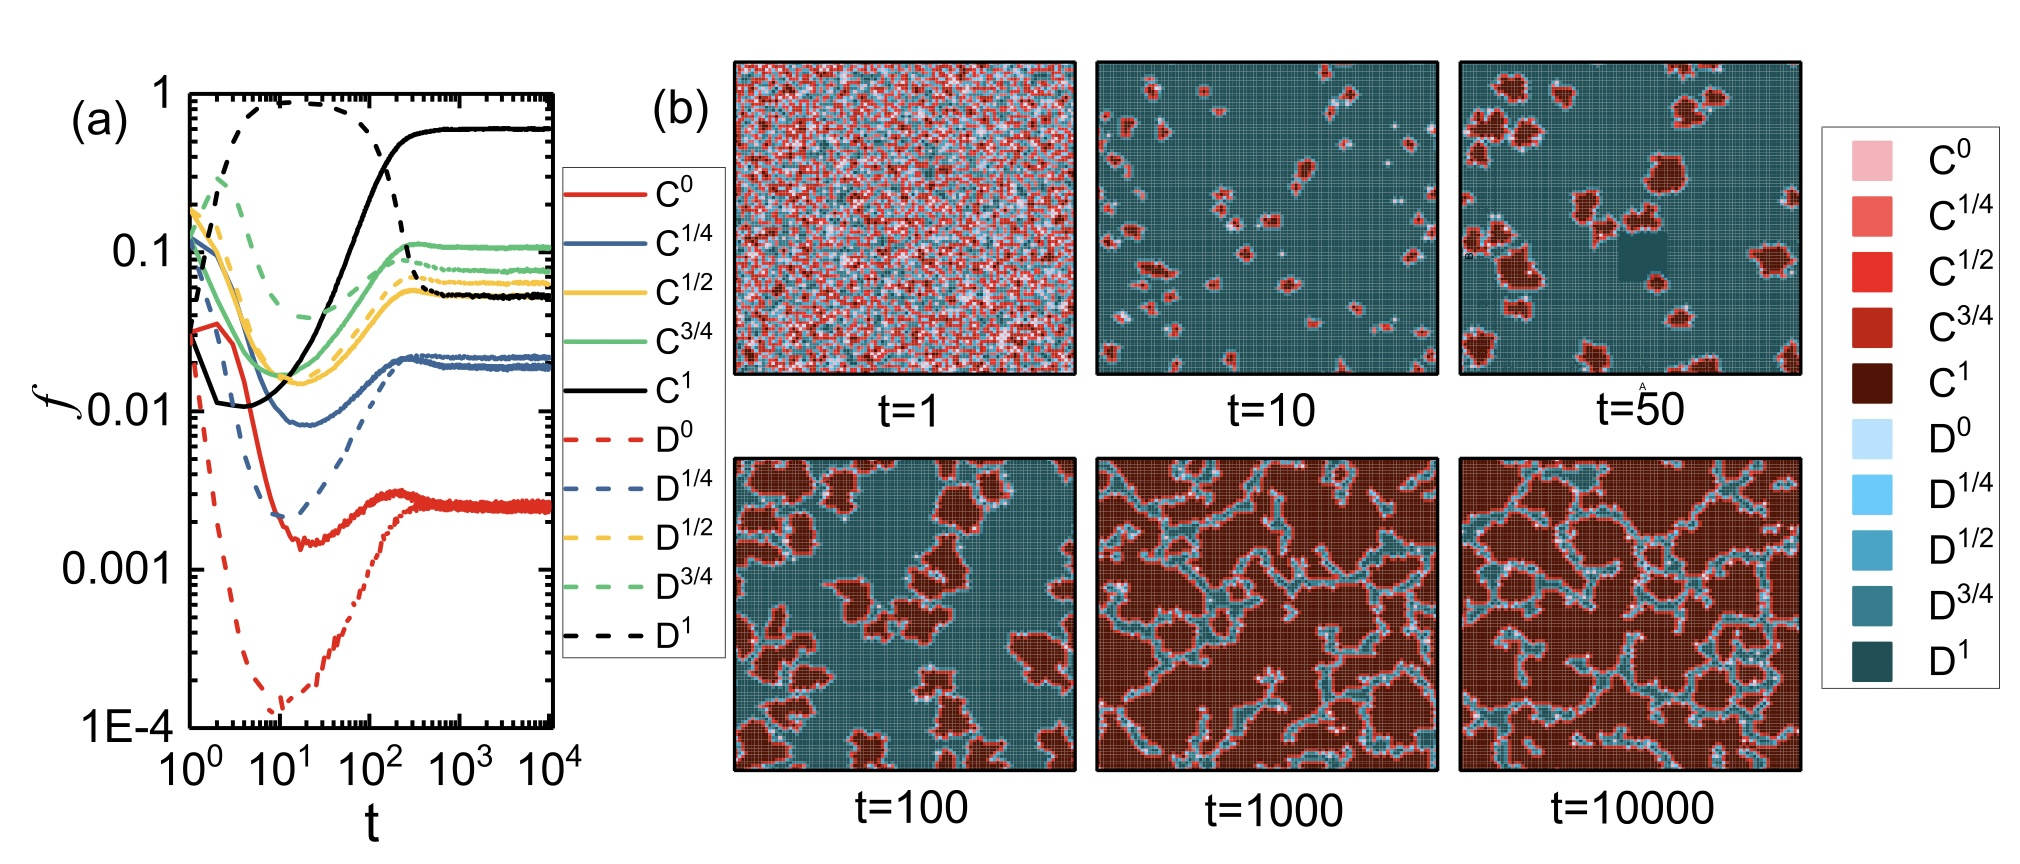
\includegraphics[width=1.05\linewidth]{5}
		\label{fig5}
		\parbox{.8\textwidth}{\scriptsize Fig\ 5 :(a) Time courses of the fractions of ten kinds of individuals. (b) Snapshots of the distributions of these ten kinds of individuals at several representative times. Other parameters: $r = 3.7$, $\alpha = 1.0$.
		}
	\end{figure}
\end{frame}


\subsection{Influence of other parameters
}
\begin{frame}{Influence of other parameters}

	\begin{figure}[H]
		\centering
		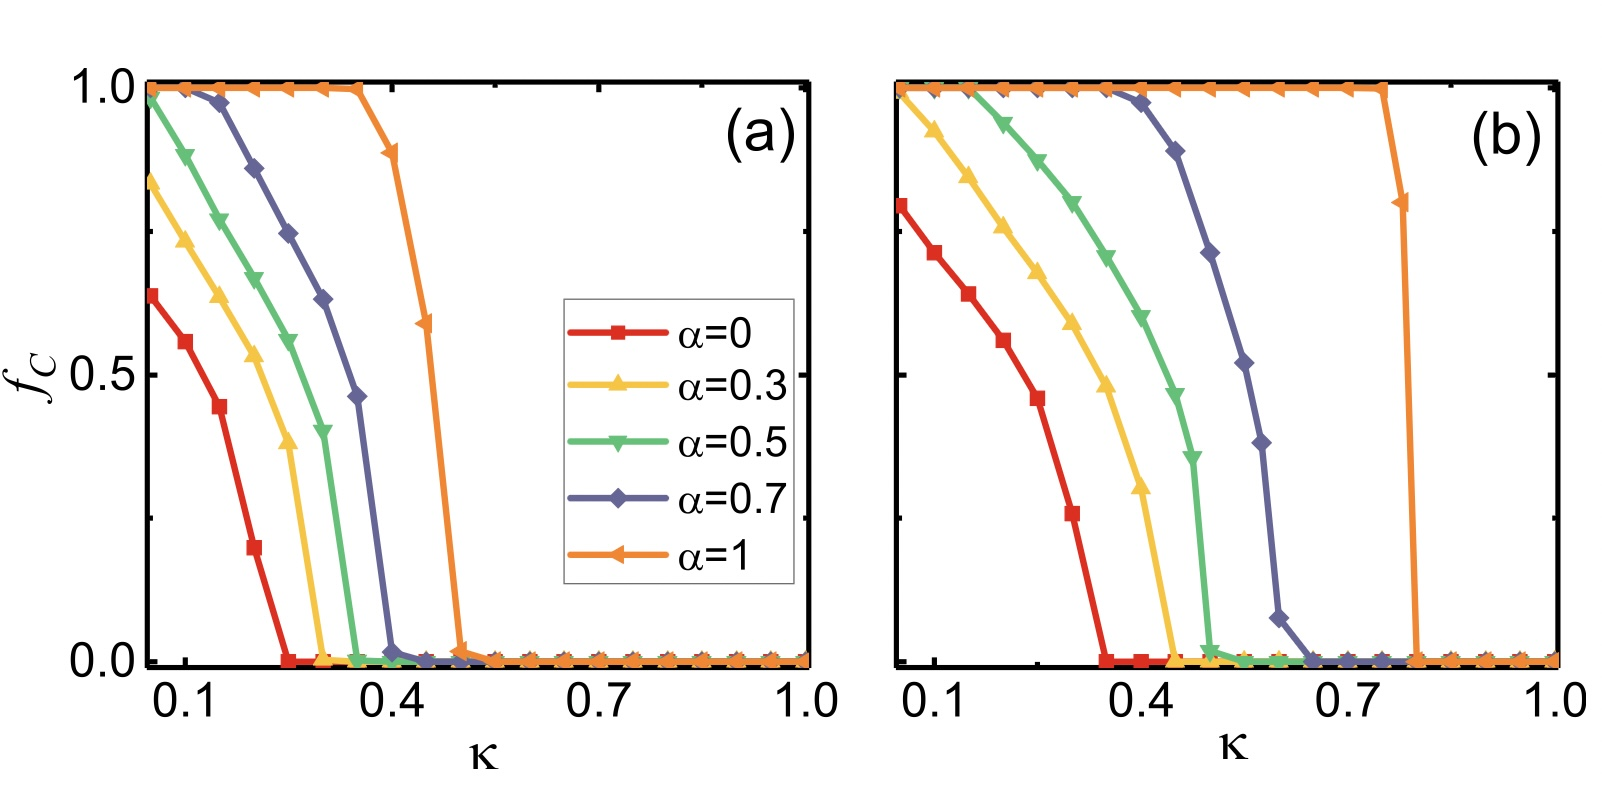
\includegraphics[width=1\linewidth]{6}
		\label{fig6}
		\parbox{.8\textwidth}{\scriptsize Fig\ 6 :Relationship between the cooperation frequency $f_C$ and the noise intensity $\kappa$ at several heterogeneity strengths $\alpha$: (a) $r = 4.2$ and (b) $r = 4.5$.}
	\end{figure}
\end{frame}


\begin{frame}{Influence of other parameters}

	\begin{figure}[H]
		\centering
		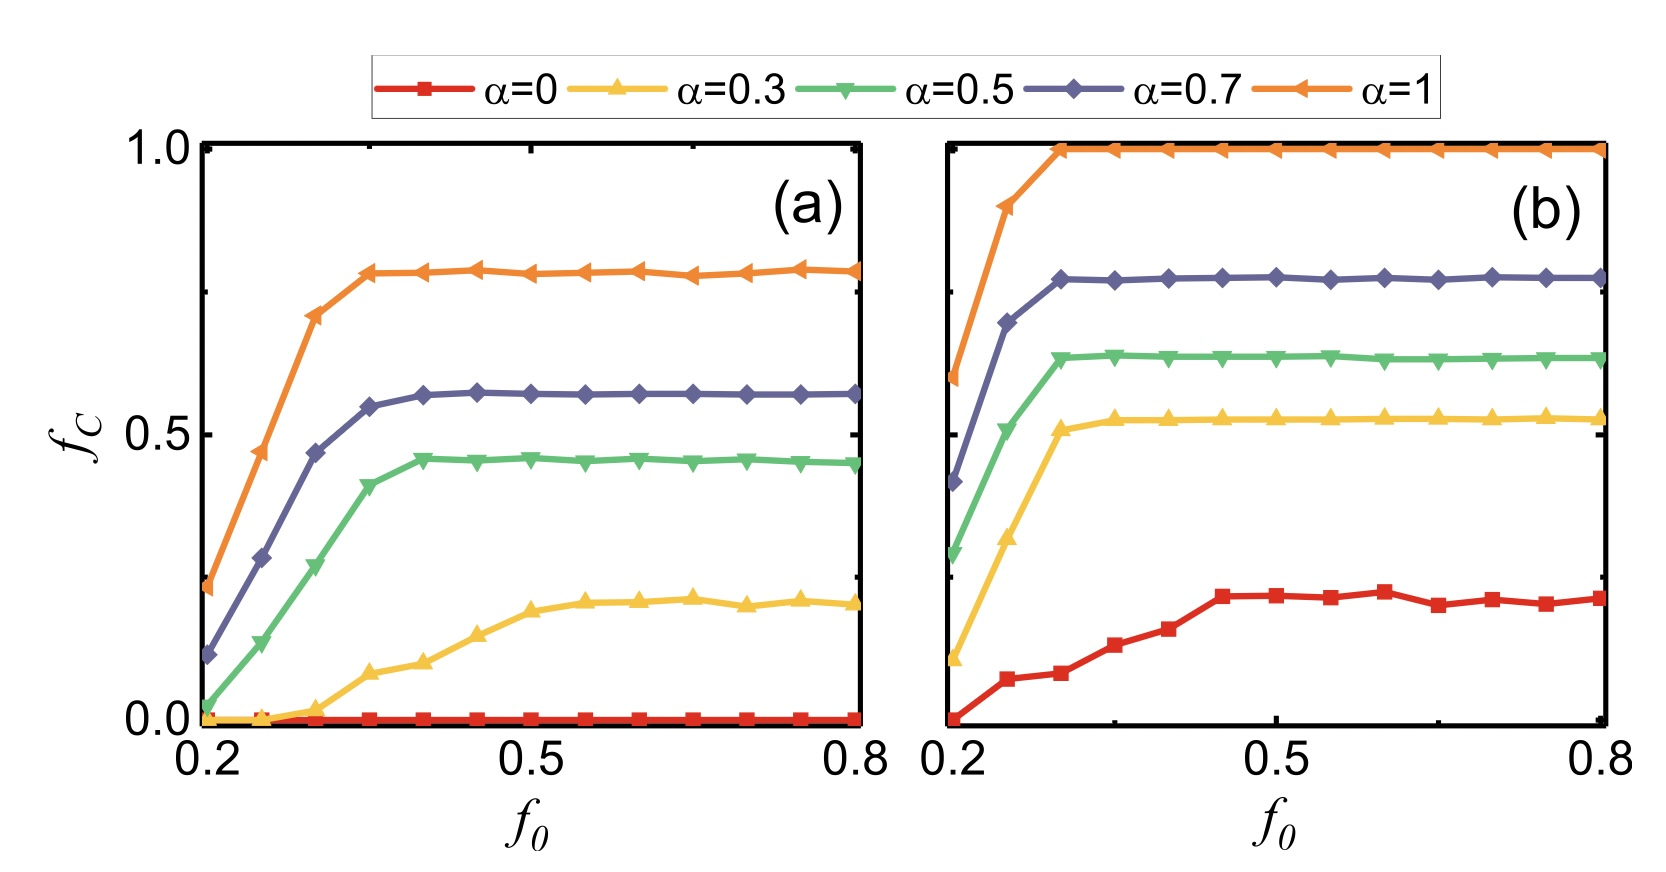
\includegraphics[width=1\linewidth]{7}
		\label{fig7}
		\parbox{.8\textwidth}{\scriptsize Fig\ 7 :Relationship between the cooperation frequency $f_C$ and the original proportion of cooperation $f_0$: (a) $r = 3.7$ and (b) $r = 3.9$.}
	\end{figure}
\end{frame}


\subsection{Robustness of the results}
\begin{frame}{Robustness of the results}
	\begin{figure}[H]
		\centering
		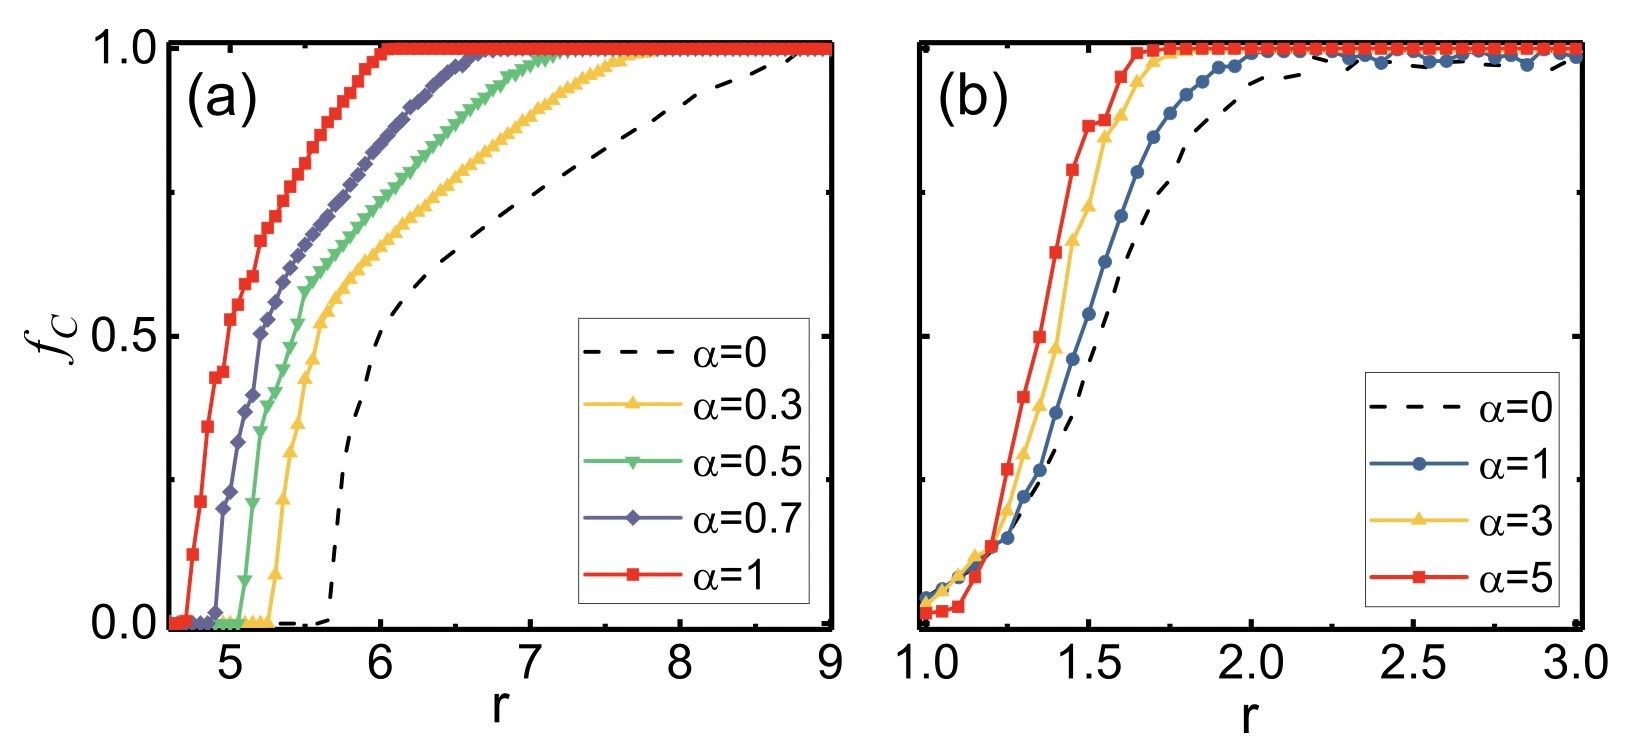
\includegraphics[width=1\linewidth]{8}
		\label{fig8}
		\parbox{.8\textwidth}{\scriptsize Fig\ 8 :Relationship between the cooperation frequency $f_C$ and the synergy factor $r$ at several heterogeneity strengths: (a) lattice with a Moore neighborhood and (b) a BA scale-free network with the average degree $\langle k\rangle = 4$.
		}
	\end{figure}
\end{frame}


\begin{frame}{Robustness of the results}
	\begin{figure}[H]
		\centering
		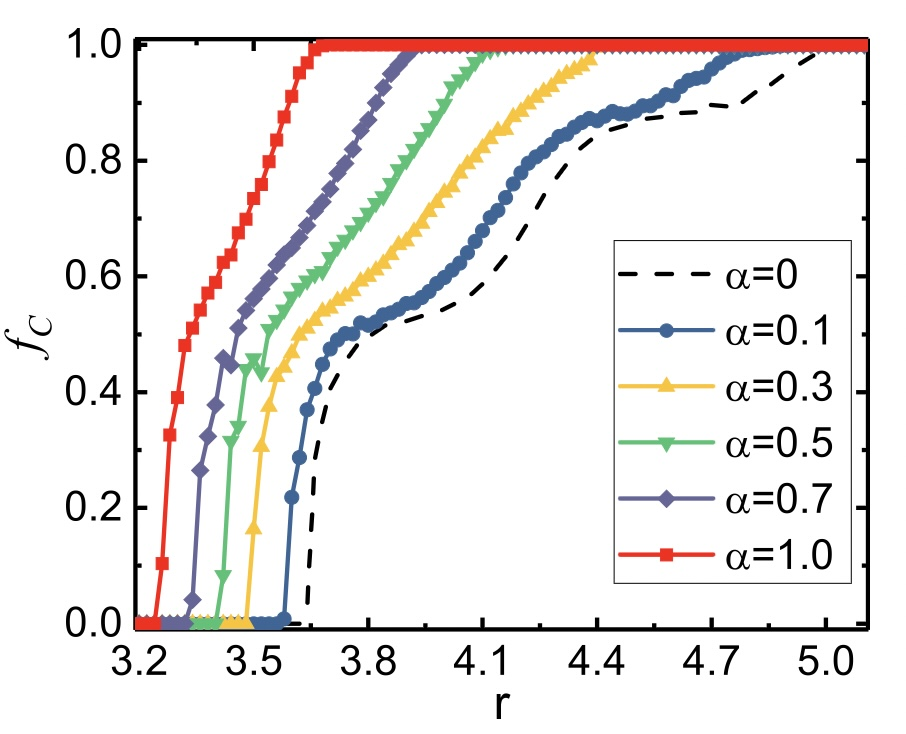
\includegraphics[width=.7\linewidth]{9}
		\label{fig9}
		\parbox{.8\textwidth}{\scriptsize Fig\ 9 :Relationship between the cooperation frequency $f_C$ and the synergy factor $r$ at several heterogeneity strengths $\alpha$ with $c = 5$.

		}
	\end{figure}
\end{frame}


%------------------------------------------------
\section{Summary and prospect}
%------------------------------------------------

\begin{frame}{Summary and prospect}

	A reputation mechanism is commonly introduced as being necessary to favor cooperation.
	In previous studies, only cooperators have been given the chance to maintain a higher reputation.

	\uline{However, this ignores the fact that some individuals in bad circumstances will be forced to defect to protect themselves against exploitation. }

	In this work, we worked on the principle that individuals who hold the same strategies as their neighbors can gain higher reputations.
	This reputation rule is introduced through heterogeneous investments to \textbf{spatial PGGs}.
	The results show that this model achieves better performance in terms of cooperative behavior, and cooperation is more favorable with stronger heterogeneity of investments.
\end{frame}


\begin{frame}{Summary and prospect}

	In this work, we found that the reputation calculation method can provide defectors in bad circumstances a higher reputation.
	It should be noted that, in this model, the reputation value depends only on the strategies chosen by each individual.
	In real-world situations, however, the reputations of individuals may be influenced by other social factors.
	In future research, a combination of strategies and other social factors could be considered.
	We hope this work contributes to the understanding of social reputation in structured populations from an evolutionary perspective.
\end{frame}

%------------------------------------------------

% \section*{}
\begin{frame}[allowframebreaks]{References}
	% \tableofcontents[sectionstyle=hide,subsectionstyle=hide]
	\printbibliography
\end{frame}



%\setbeamertemplate{headline}{}
\begin{frame}
	%\sffamily
	\begin{center}
		{\textcolor[RGB]{165,3,3}{\fontsize{60}{0}\selectfont
				% 谢\quad 谢! \\[8pt]
				Thank you!}}
	\end{center}
\end{frame}

\end{document}
